\documentclass[a4j,12pt,]{jarticle}
 \usepackage{float}
 \usepackage{siunitx} %%SI単位系用
 \usepackage{amssymb, amsmath}
 \usepackage{ascmac,here,txfonts}
 \usepackage{hyperref}
 \usepackage{listings}
 \usepackage{pxjahyper}
 \usepackage[dvipdfmx]{graphicx}
 \usepackage{amssymb, amsmath}
  \usepackage{listings}
  \usepackage[dvipdfmx]{color}

  \lstset{
    language={Python},
    basicstyle={\ttfamily},
    identifierstyle={\small},
    commentstyle={\small\itshape},
    keywordstyle={\small\bfseries},
    ndkeywordstyle={\small},
    stringstyle={\small\ttfamily},
    frame={single},
    breaklines=true,
    columns=[l]{fullflexible},
    numbers=left,
    xrightmargin=0zw,
    xleftmargin=3zw,
    numberstyle={\scriptsize},
    stepnumber=1,
    numbersep=1zw,
    lineskip=-0.5ex,
  }

\begin{document}

{\noindent\small 第22回報告書 \hfill\today}
\begin{center}
  {\Large 異なるElasticsearchクラスタへのノード参加検証}
\end{center}
\begin{flushright}
  祖父江匠真 \\
\end{flushright}

\section{概要}
今回は, CO\textsubscript{2}データなどが保存されている3ノードで構築されたクラスタに対して, リサイクル館の太陽光パネルの計測データを保存しているElasticsearchノードが新たなノードとしてクラスタに参加できるか, Dockerを用いて検証した.

\section{手順}

\subsection{単一ノードで稼働するクラスタAの構築とシャットダウン}

まず, docker-composeを用いて単一ノード(コンテナ名はes04)でクラスタ(以後このクラスタをクラスタAと呼ぶ)を構築する.

Listing \ref{sc1}にクラスタAの構築の際に使用したdocker-compose.ymlを示す.

% \begin{figure}[H]
%   \begin{center}
%     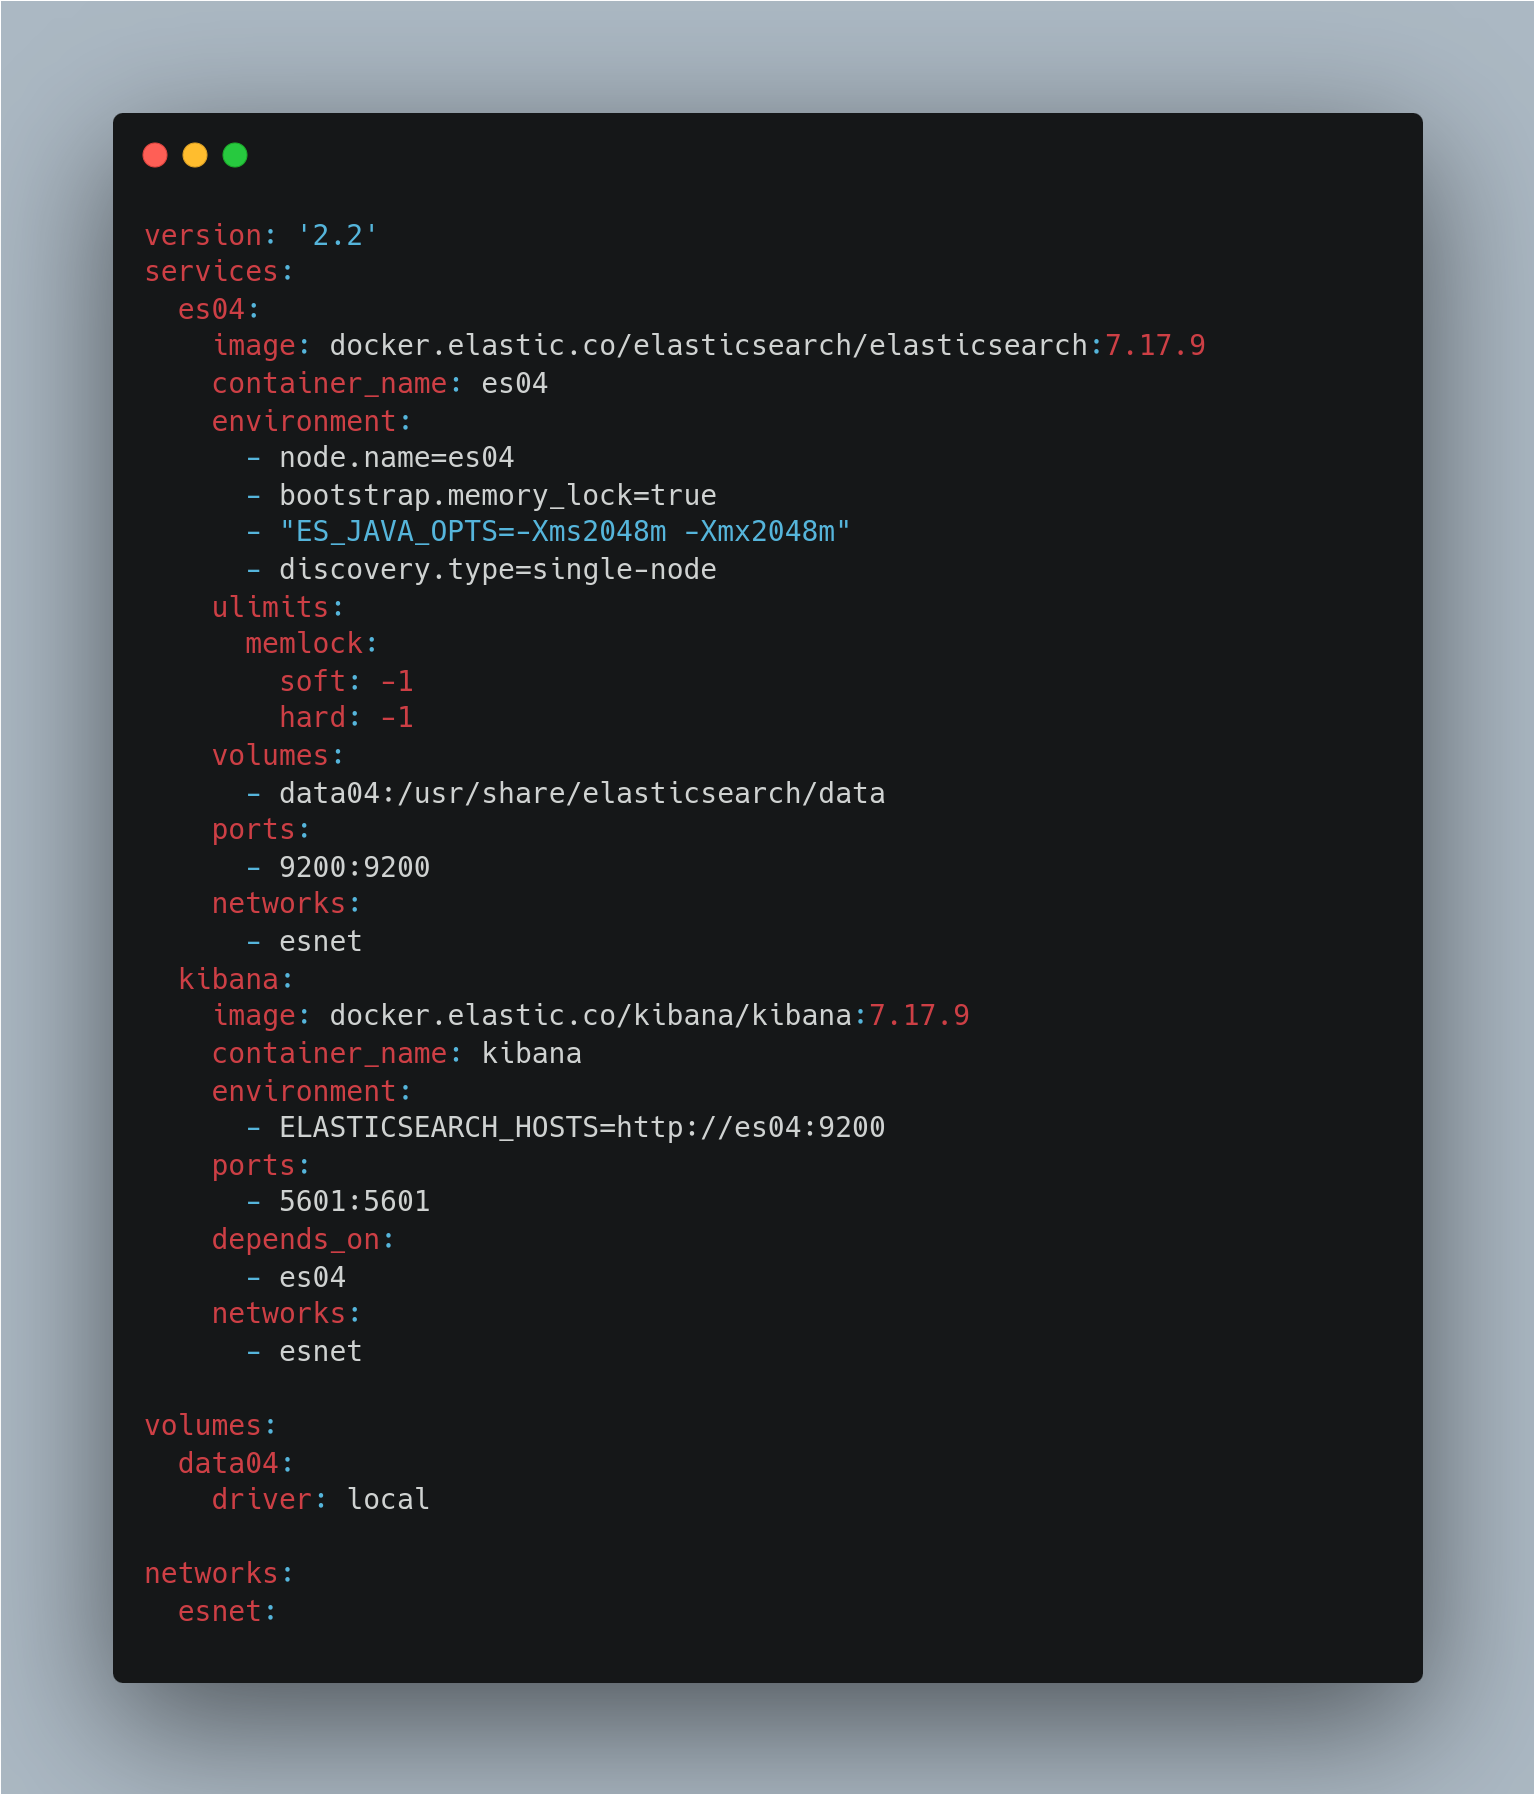
\includegraphics[width=160mm]{es04.png}
%     \caption{クラスタAの構築の際に使用したdocker-compose.yml}
%     \label{p1}
%   \end{center}
% \end{figure}

\begin{lstlisting}[caption=クラスタAの構築の際に使用したdocker-compose.yml, label=sc1]
version: '2.2'
services:
  es04:
    image: docker.elastic.co/elasticsearch/elasticsearch:7.17.9
    container_name: es04
    environment:
      - node.name=es04
      - bootstrap.memory_lock=true
      - "ES_JAVA_OPTS=-Xms2048m -Xmx2048m"
      - discovery.type=single-node
    volumes:
      - data04:/usr/share/elasticsearch/data
    ports:
      - 9200:9200
    networks:
      - esnet

volumes:
  data04:
    driver: local

networks:
  esnet:
\end{lstlisting}

docker-composeを用いてノードを起動した後, クラスタの情報について問い合わせた結果を図 \ref{p1-1}に示す.

\begin{figure}[H]
  \begin{center}
    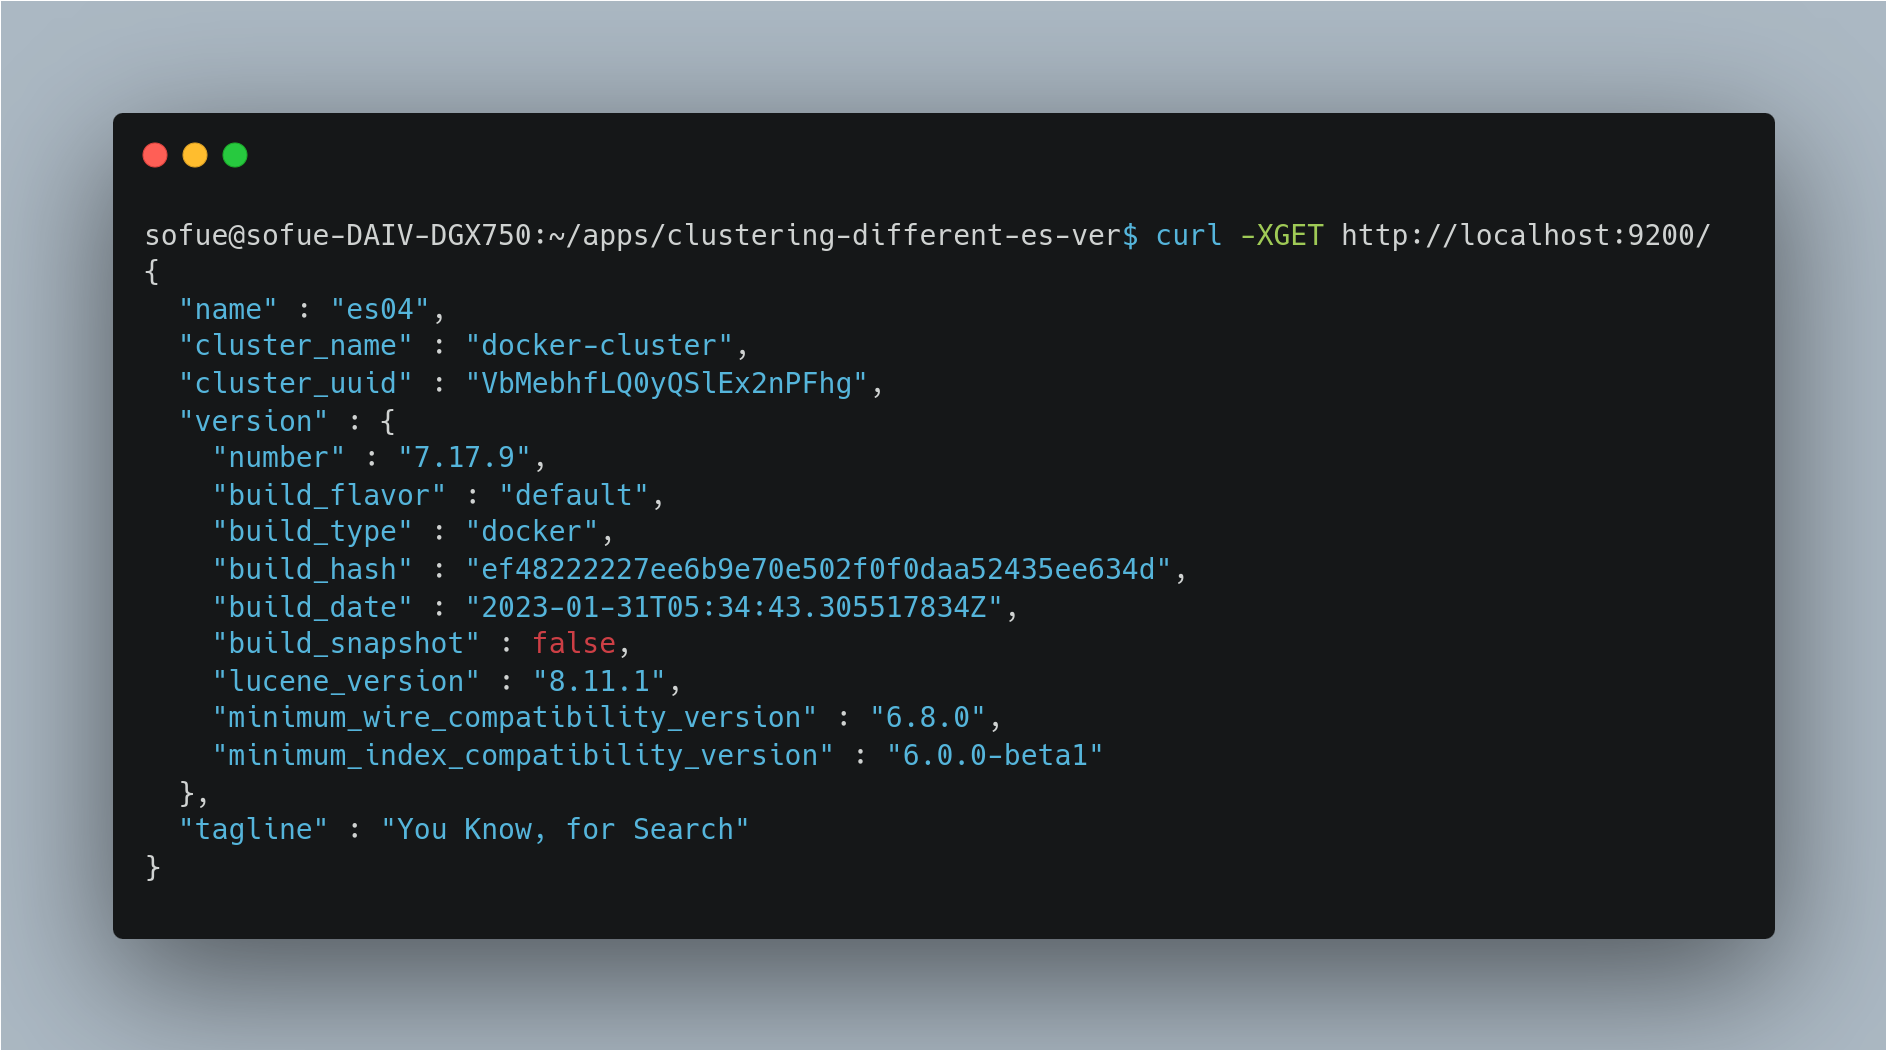
\includegraphics[width=160mm]{es04-cluster.png}
    \caption{クラスタの情報について問い合わせた結果}
    \label{p1-1}
  \end{center}
\end{figure}

最後にノードをシャットダウンした.

\subsection{クラスタBの構築とシャットダウン}

次に, クラスタAに使用したノードとは別の3ノード(コンテナ名はそれぞれes01, es02, es03)でクラスタ(以後このクラスタをクラスタBと呼ぶ)を構築する.

Listing \ref{sc2}にクラスタBの構築の際に使用したdocker-compose.ymlを示す.

% \begin{figure}[H]
%   \begin{center}
%     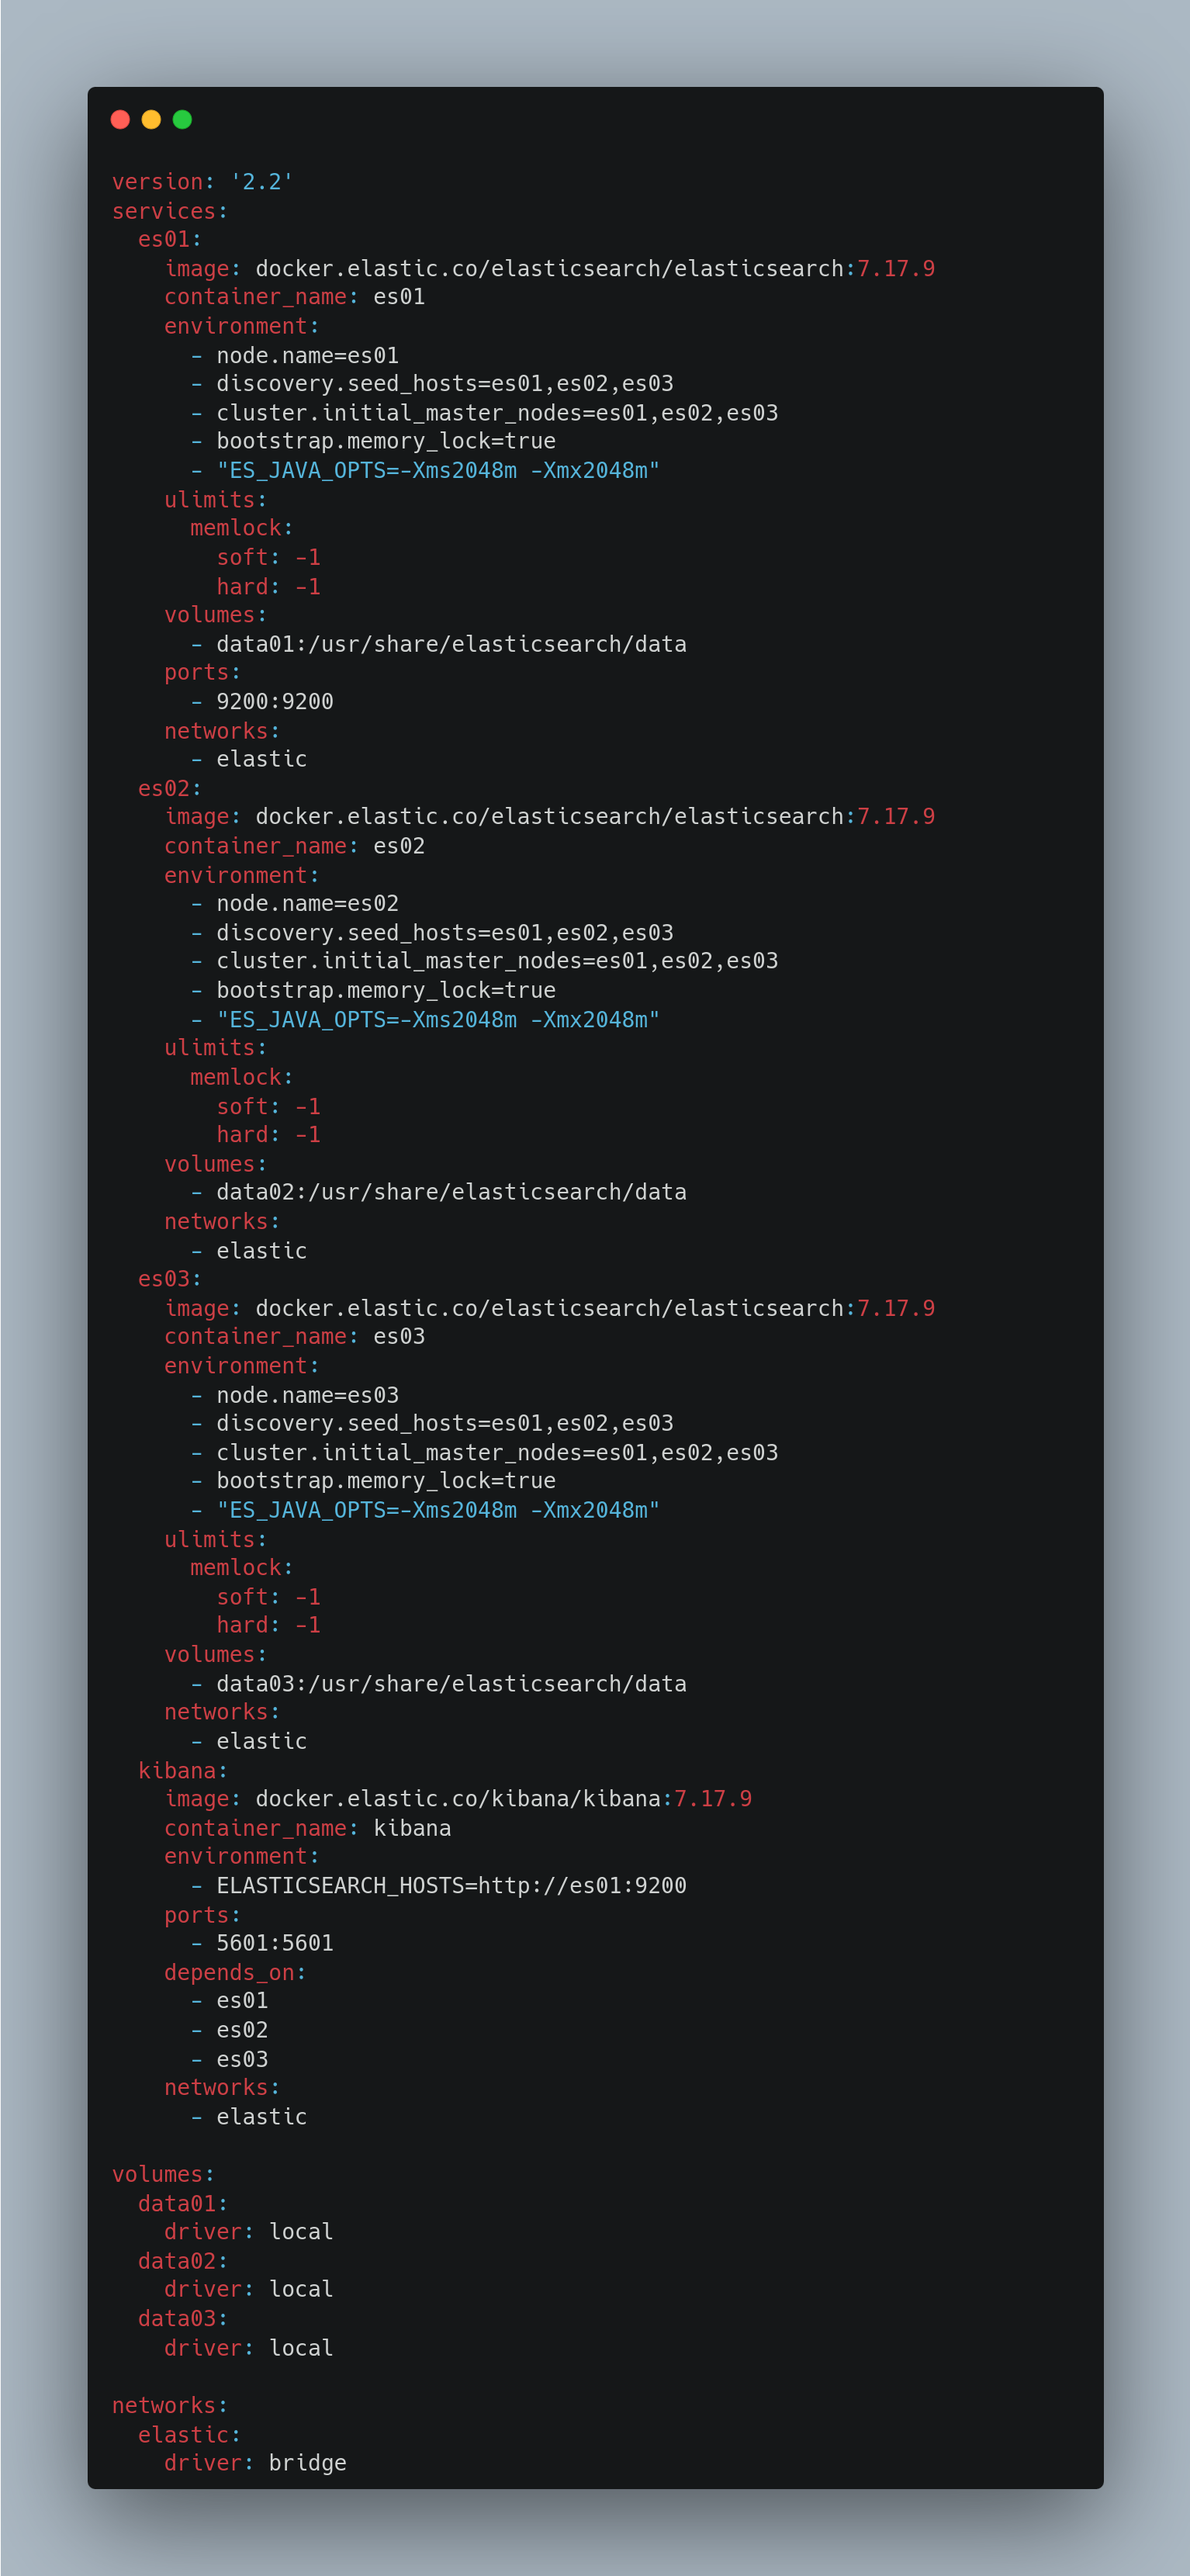
\includegraphics[width=160mm]{3nodes.png}
%     \caption{クラスタBの構築の際に使用したdocker-compose.yml}
%     \label{p2}
%   \end{center}
% \end{figure}

\begin{lstlisting}[caption=クラスタBの構築の際に使用したdocker-compose.yml, label=sc2]
version: '2.2'
services:
  es01:
    image: docker.elastic.co/elasticsearch/elasticsearch:7.17.9
    container_name: es01
    environment:
      - node.name=es01
      - discovery.seed_hosts=es01,es02,es03
      - cluster.initial_master_nodes=es01,es02,es03
      - bootstrap.memory_lock=true
      - "ES_JAVA_OPTS=-Xms2048m -Xmx2048m"
    volumes:
      - data01:/usr/share/elasticsearch/data
    ports:
      - 9200:9200
    networks:
      - elastic
  es02:
    image: docker.elastic.co/elasticsearch/elasticsearch:7.17.9
    container_name: es02
    environment:
      - node.name=es02
      - discovery.seed_hosts=es01,es02,es03
      - cluster.initial_master_nodes=es01,es02,es03
      - bootstrap.memory_lock=true
      - "ES_JAVA_OPTS=-Xms2048m -Xmx2048m"
    volumes:
      - data02:/usr/share/elasticsearch/data
    networks:
      - elastic
  es03:
    image: docker.elastic.co/elasticsearch/elasticsearch:7.17.9
    container_name: es03
    environment:
      - node.name=es03
      - discovery.seed_hosts=es01,es02,es03
      - cluster.initial_master_nodes=es01,es02,es03
      - bootstrap.memory_lock=true
      - "ES_JAVA_OPTS=-Xms2048m -Xmx2048m"
    volumes:
      - data03:/usr/share/elasticsearch/data
    networks:
      - elastic

volumes:
  data01:
    driver: local
  data02:
    driver: local
  data03:
    driver: local

networks:
  elastic:
    driver: bridge
\end{lstlisting}

docker-composeを用いて3つのノードを起動した後, クラスタの情報について問い合わせた結果を図 \ref{p2-1}に示す.

\begin{figure}[H]
  \begin{center}
    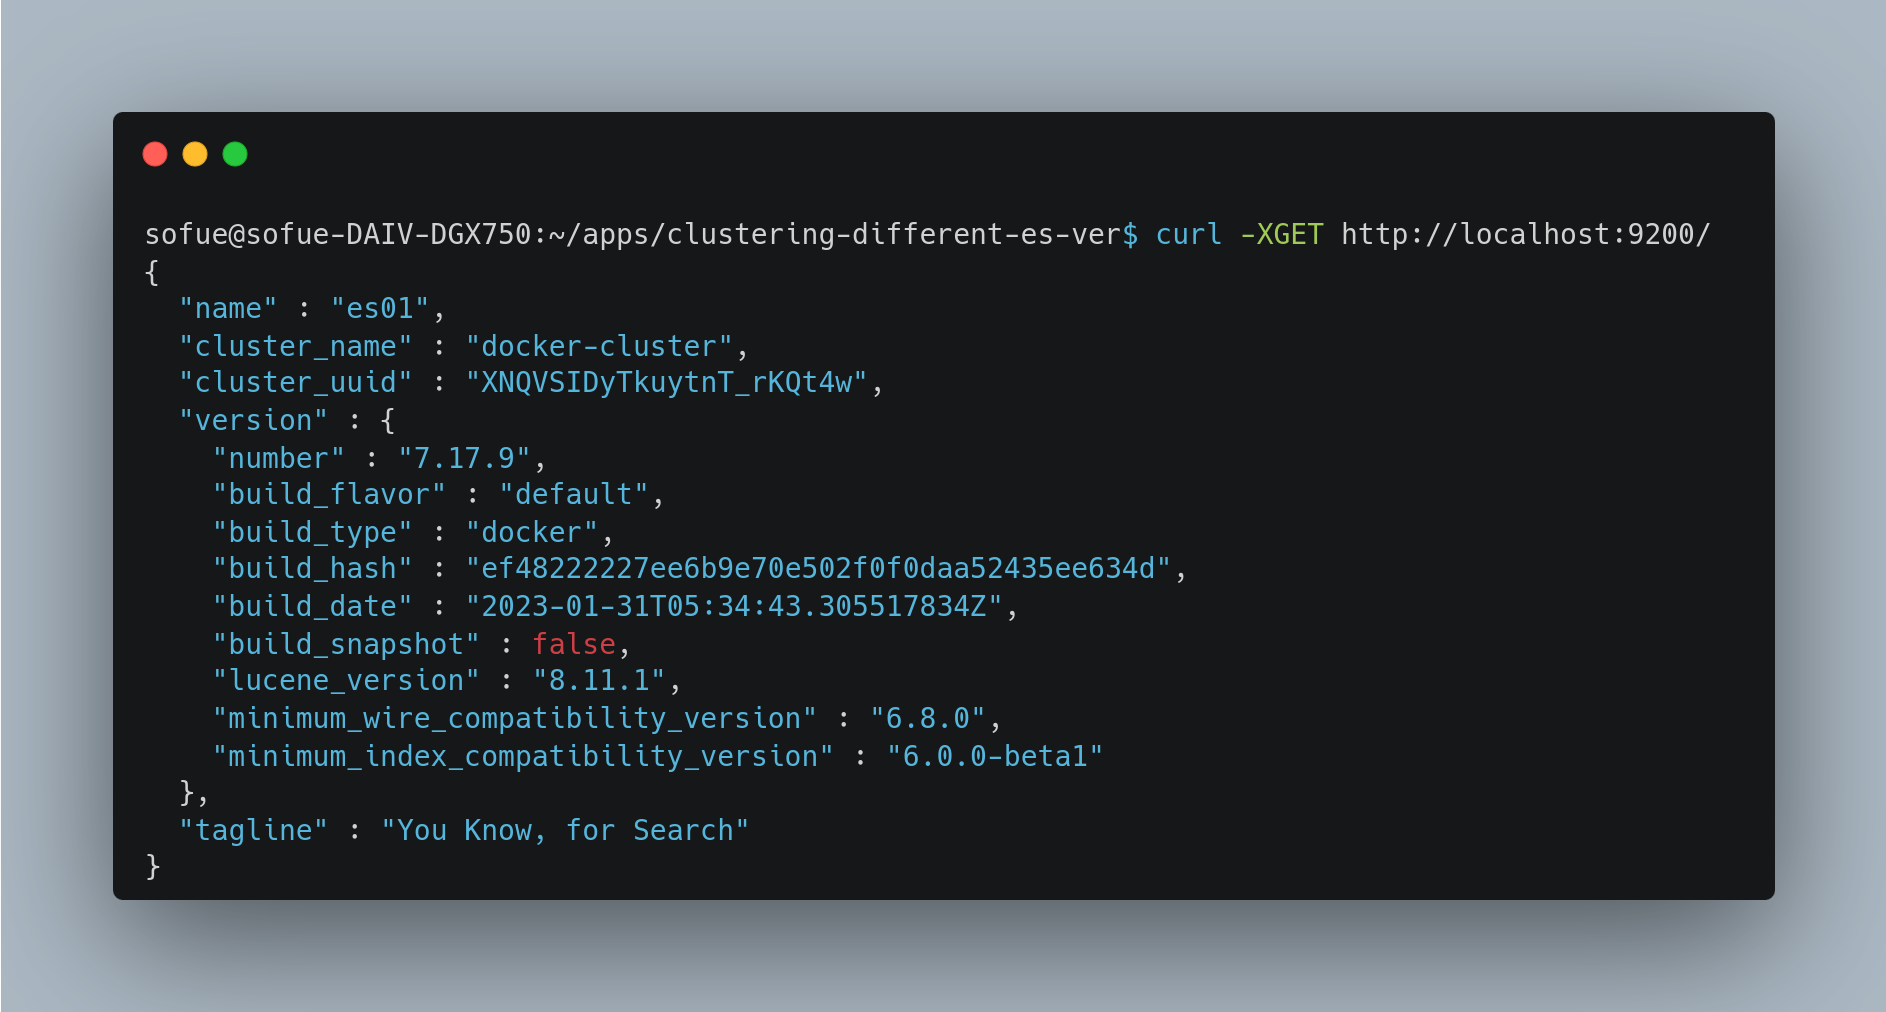
\includegraphics[width=160mm]{3nodes-cluster.png}
    \caption{クラスタの情報について問い合わせた結果}
    \label{p2-1}
  \end{center}
\end{figure}

最後にノードを全てシャットダウンした.

\subsection{クラスタBへの参加試行}

次に, Listing \ref{sc2}のdocker-compose.ymlに, クラスタAのノード(es04)を追加し, 合計4ノードでクラスタBを起動する.

Listing \ref{sc3}に, 合計4ノードでクラスタBを起動する際に使用したdocker-compose.ymlを示す.

\begin{figure}[H]
  \begin{center}
    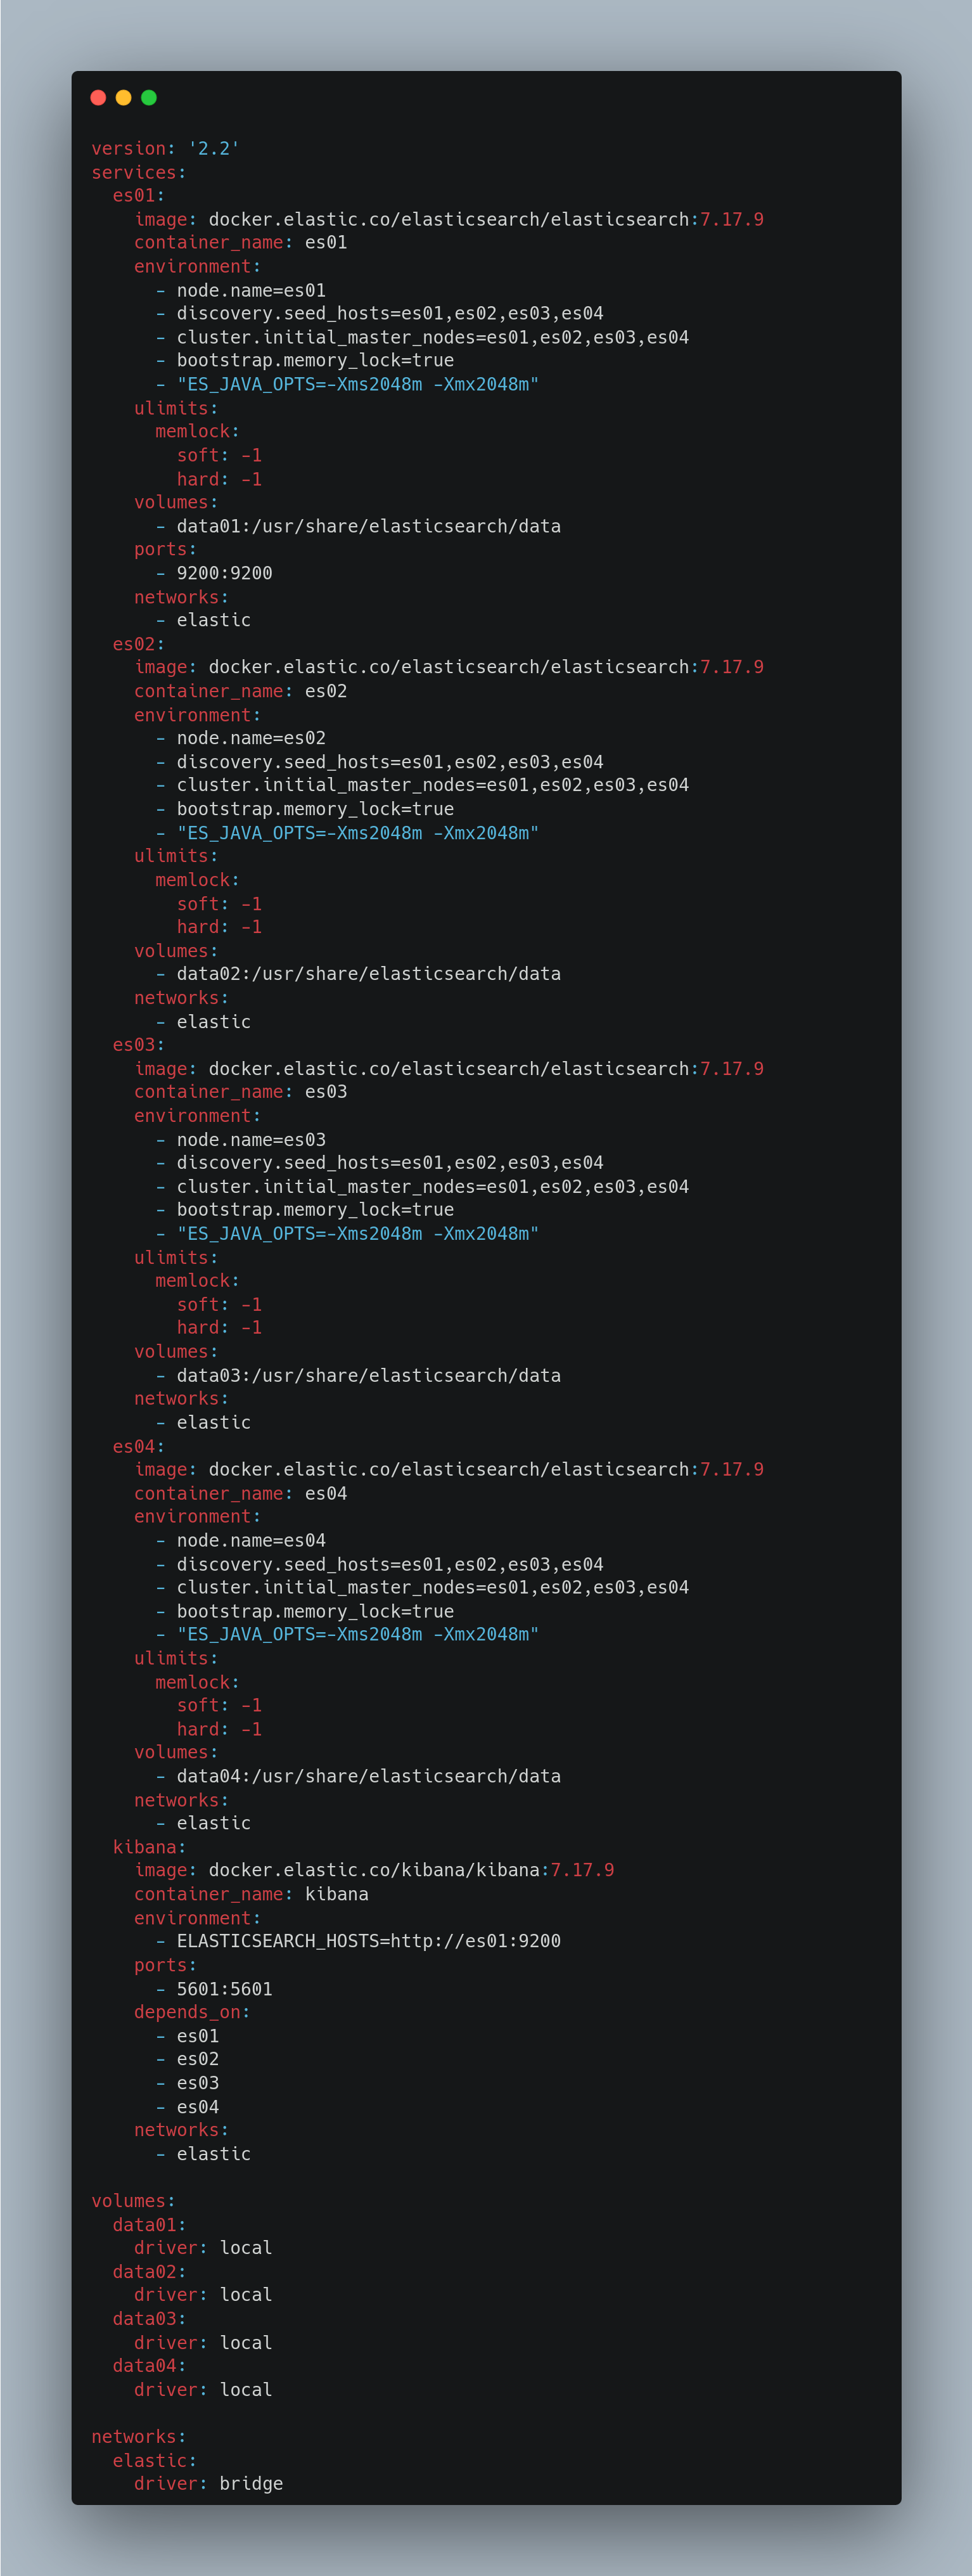
\includegraphics[width=160mm]{4nodes.png}
    \caption{合計4ノードでクラスタBを起動する際に使用したdocker-compose.yml}
    \label{p3}
  \end{center}
\end{figure}

\begin{lstlisting}[caption=合計4ノードでクラスタBを起動する際に使用したdocker-compose.yml, label=sc3]
version: '2.2'
services:
  es01:
    image: docker.elastic.co/elasticsearch/elasticsearch:7.17.9
    container_name: es01
    environment:
      - node.name=es01
      - discovery.seed_hosts=es01,es02,es03,es04
      - cluster.initial_master_nodes=es01,es02,es03,es04
      - bootstrap.memory_lock=true
      - "ES_JAVA_OPTS=-Xms2048m -Xmx2048m"
    volumes:
      - data01:/usr/share/elasticsearch/data
    ports:
      - 9200:9200
    networks:
      - elastic
  es02:
    image: docker.elastic.co/elasticsearch/elasticsearch:7.17.9
    container_name: es02
    environment:
      - node.name=es02
      - discovery.seed_hosts=es01,es02,es03,es04
      - cluster.initial_master_nodes=es01,es02,es03,es04
      - bootstrap.memory_lock=true
      - "ES_JAVA_OPTS=-Xms2048m -Xmx2048m"
    volumes:
      - data02:/usr/share/elasticsearch/data
    networks:
      - elastic
  es03:
    image: docker.elastic.co/elasticsearch/elasticsearch:7.17.9
    container_name: es03
    environment:
      - node.name=es03
      - discovery.seed_hosts=es01,es02,es03,es04
      - cluster.initial_master_nodes=es01,es02,es03,es04
      - bootstrap.memory_lock=true
      - "ES_JAVA_OPTS=-Xms2048m -Xmx2048m"
    volumes:
      - data03:/usr/share/elasticsearch/data
    networks:
      - elastic
  es04:
    image: docker.elastic.co/elasticsearch/elasticsearch:7.17.9
    container_name: es04
    environment:
      - node.name=es04
      - discovery.seed_hosts=es01,es02,es03,es04
      - cluster.initial_master_nodes=es01,es02,es03,es04
      - bootstrap.memory_lock=true
      - "ES_JAVA_OPTS=-Xms2048m -Xmx2048m"
    volumes:
      - data04:/usr/share/elasticsearch/data
    networks:
      - elastic

volumes:
  data01:
    driver: local
  data02:
    driver: local
  data03:
    driver: local
  data04:
    driver: local

networks:
  elastic:
    driver: bridge
  \end{lstlisting}

クラスタの起動後, クラスタに参加しているノードの一覧を取得した結果を図 \ref{p3-1}に示す.

\begin{figure}[H]
  \begin{center}
    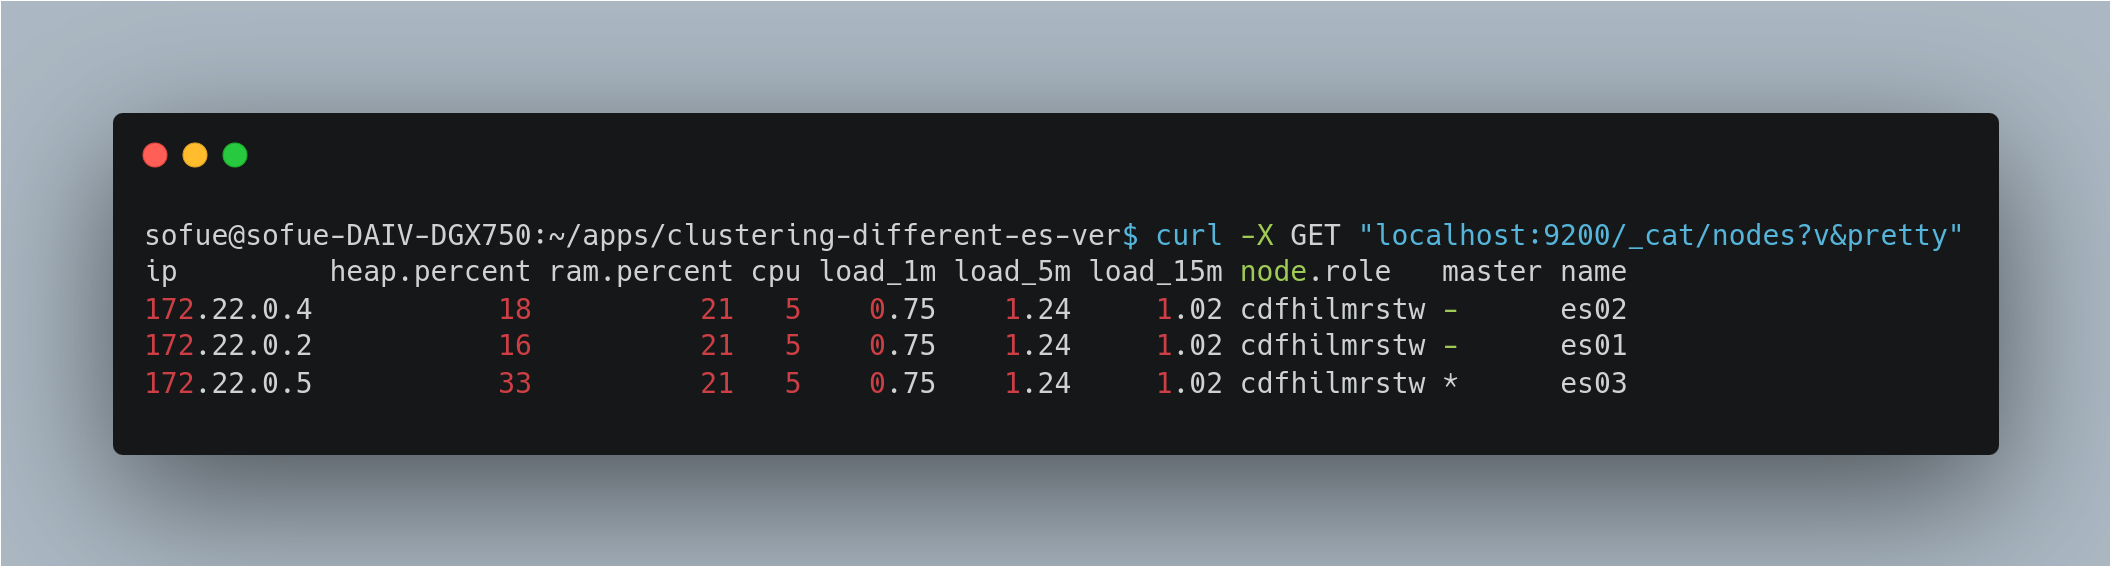
\includegraphics[width=160mm]{4nodes-list.png}
    \caption{合計4ノードでクラスタを起動した後, クラスタに参加しているノードの一覧を取得した結果}
    \label{p3-1}
  \end{center}
\end{figure}

図 \ref{p3-1}より, クラスタAのノードがクラスタBに参加できていないことが分かる.

es04コンテナ(クラスタAのノード)で出力されたログの一部を図 \ref{p3-2}に示す.

\begin{figure}[H]
  \begin{center}
    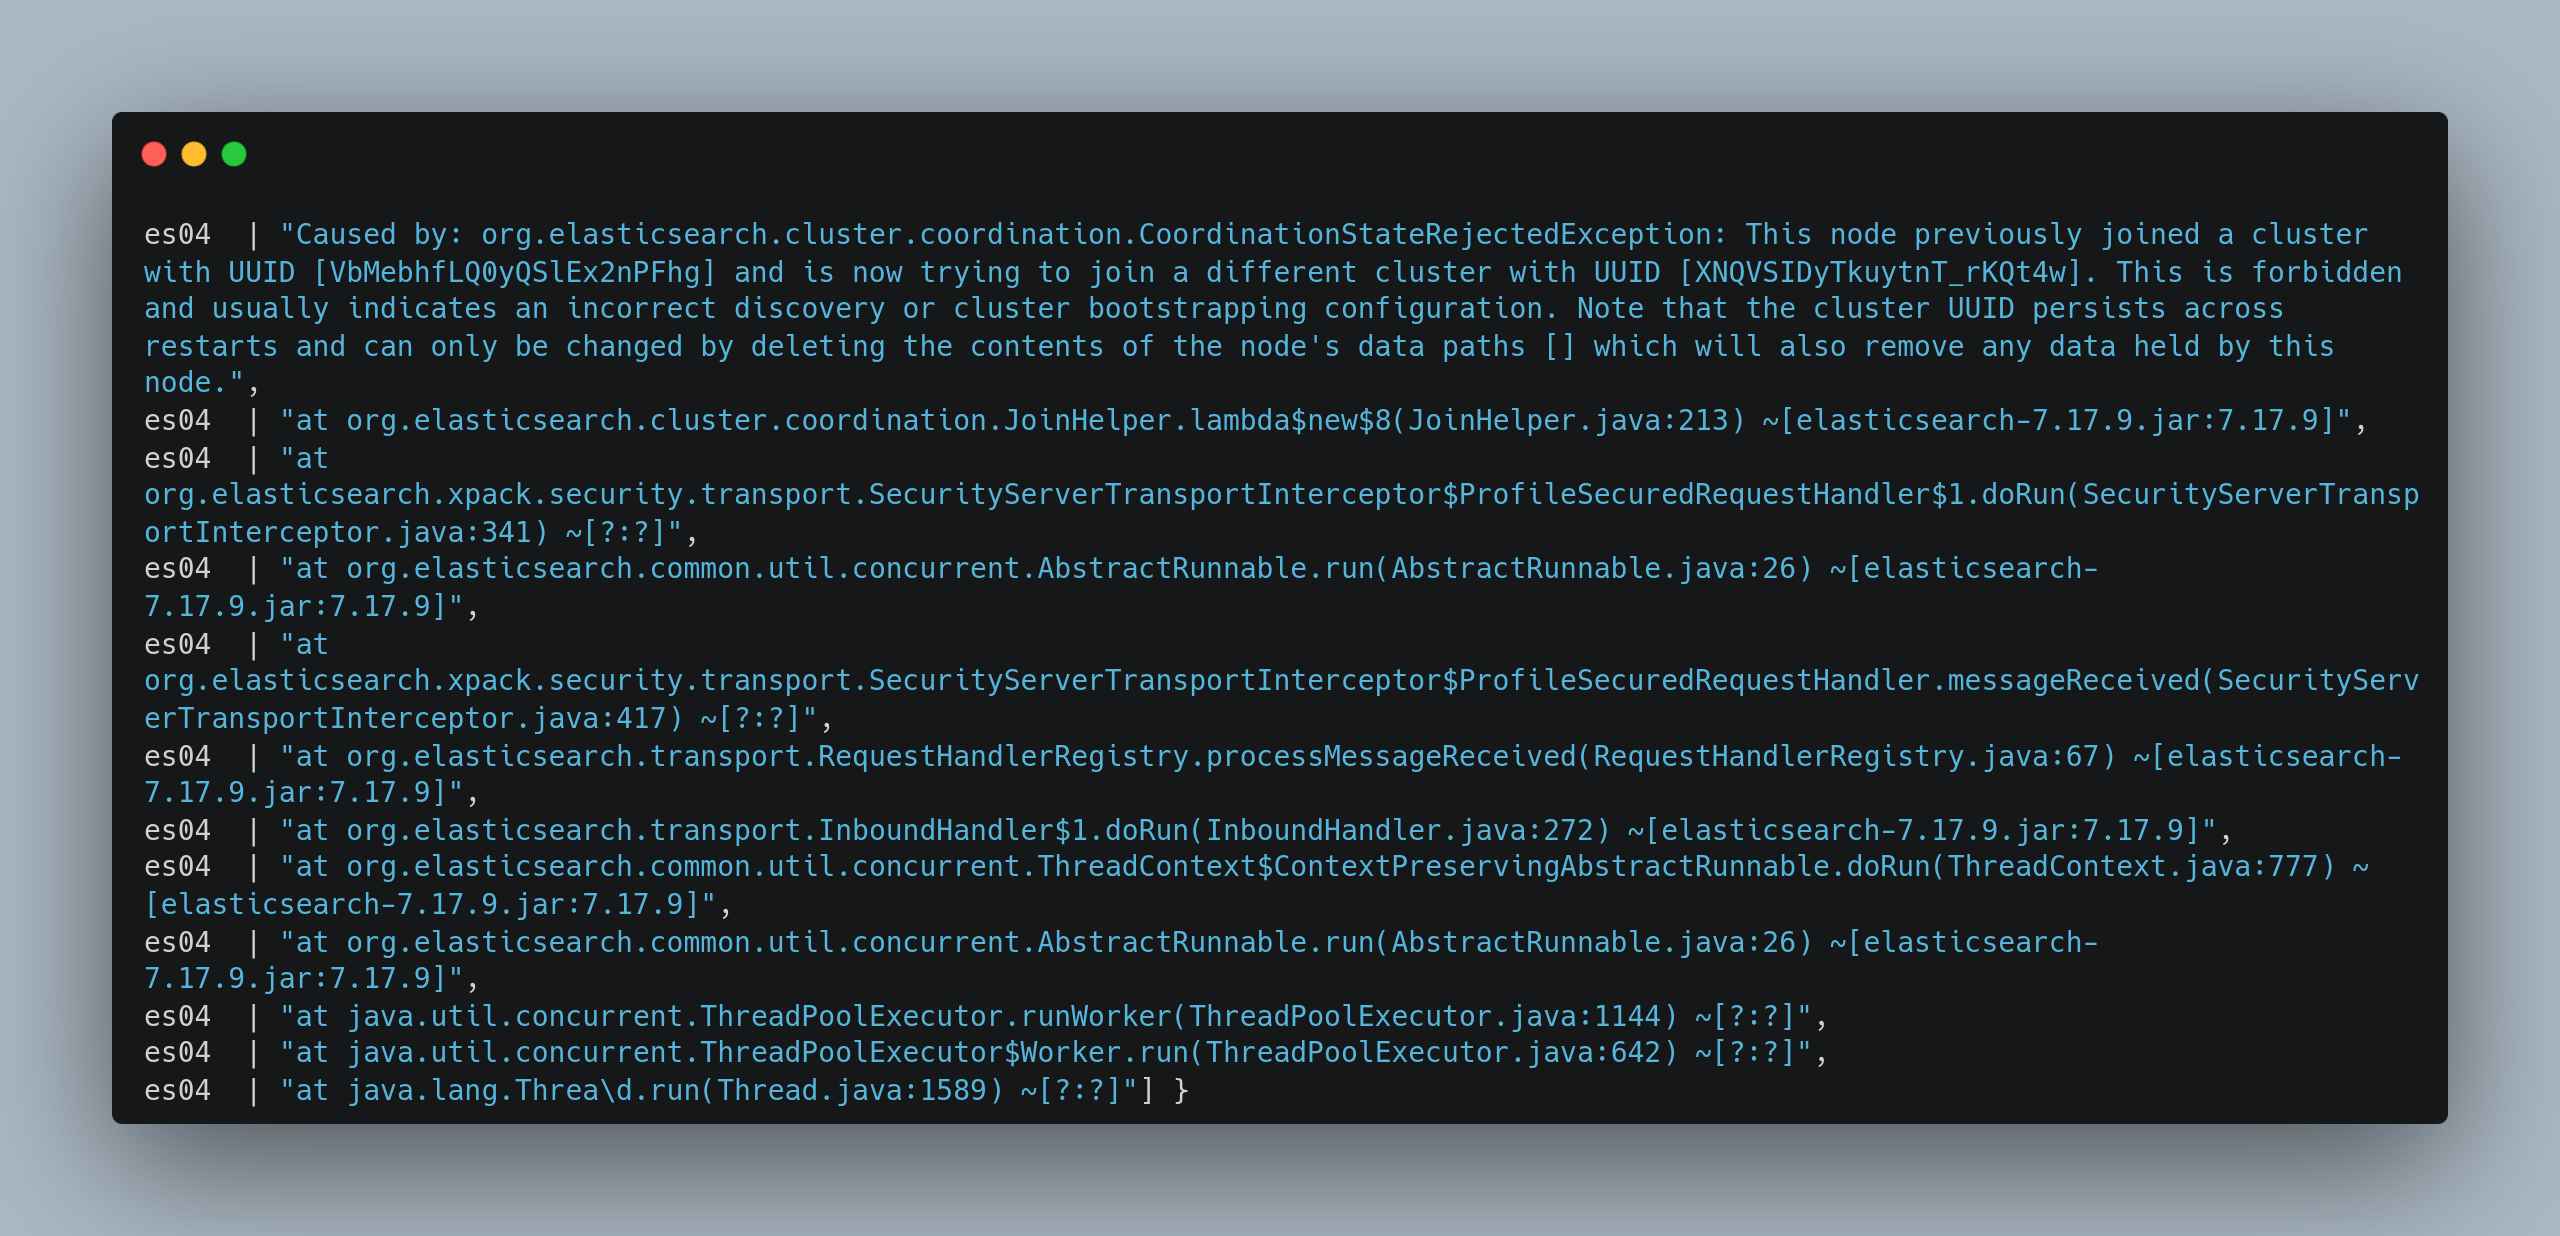
\includegraphics[width=160mm]{es04-log.png}
    \caption{es04コンテナのログ}
    \label{p3-2}
  \end{center}
\end{figure}

図 \ref{p3-2}には, 異なるクラスタIDを持つクラスタにノードが参加することは禁止されており, これを行うためにはインデックスやドキュメント情報などが格納されているデータパス配下のフォルダ, ファイルを削除する必要があると書かれている.

以上の検証結果から, 既に稼働しているノードを別のクラスタに新しいノードとして参加させることは出来ないことが分かった.

\section{まとめ}
今回は, CO\textsubscript{2}データなどが保存されている3ノードで構築されたクラスタに対して, リサイクル館の太陽光パネルの計測データを保存しているElasticsearchノードが新たなノードとしてクラスタに参加できるか, Dockerを用いて検証した.

検証の結果, Elasticsearchのノードは異なるクラスタIDを持つクラスタに参加することはできないことが分かった.ノードが別のクラスタに参加するためには, インデックスやドキュメント情報などを格納しているデータパスのフォルダやファイルを削除する必要があるが, これはそのノードのデータを失うことを意味する.

したがって, リサイクル館の太陽光パネルの計測データが保存されたElasticsearchノードをクラスタに参加させるには以下の2通りの方法が考えられる.

1. リサイクル館の太陽光パネルの計測データが保存されたElasticsearchノードのバックアップを取り, ノードに保存されたインデックスやドキュメントのデータを削除した上で, CO\textsubscript{2}データなどが保存されたクラスタに新しいノードとして参加させる
2. CO\textsubscript{2}データなどが保存されたクラスタとは別で, サーバーゾーンに新たにクラスタを構築する.

\begin{thebibliography}{5}
  \bibitem{1}Elasticsearch B.V., ”Data node's cluster uuid diffrent from master node's cluster uuid”, https://discuss.elastic.co/t/data-node-s-cluster-uuid-diffrent-from-master-nodes-cluster-uuid/196737, 参照 Dec 18,2023.
\end{thebibliography}

\end{document}

